\section{Introduction}
\label{sec:intro}

Distributed robotic applications have significant potential in transforming manufacturing, transportation, delivery, surveillance, and mapping~\cite{}. Following the trends in the cloud, mobile, and machine learning applications, programmability is going to be important in unlocking this potential  as platforms become more open and hardware developers shift to the applications marketplace. Unfortunately, domain specific languages (DSL) for robotics are surgically platform dependent, and they combine low-level sensing, communication, and control tasks with the application-level logic~\cite{}. This tight-coupling of applications with platform-specfic details can hinder development, modularity, portability, code reuse, and testing.


\begin{figure}[h!]
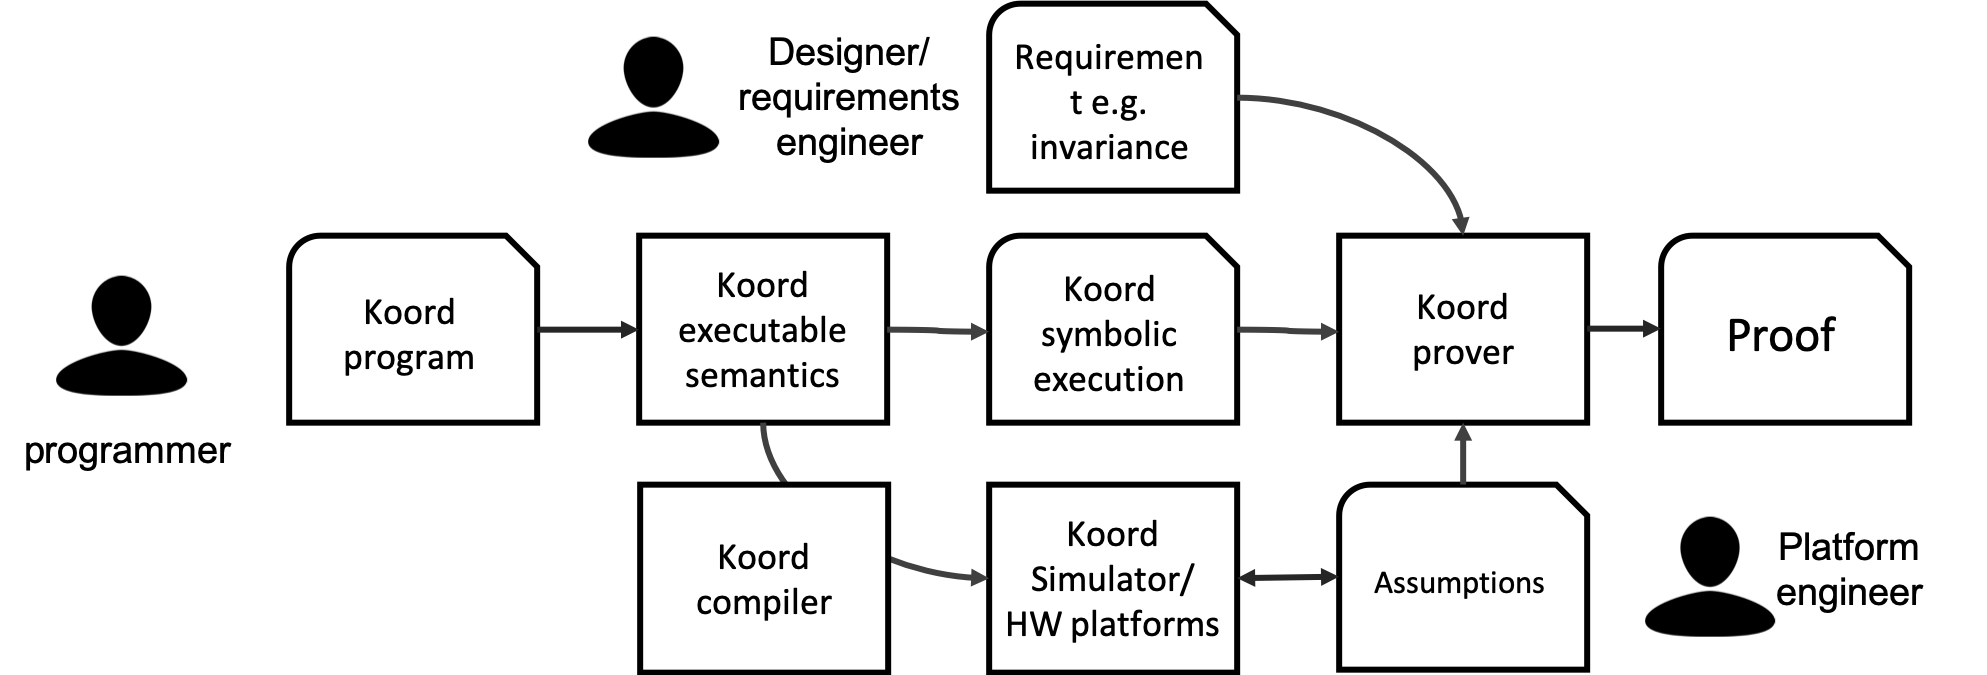
\includegraphics[width=\linewidth]{figs/koorduser.png}
\caption{\small \lgname language  enables programmers to develop distributed robotics applications using a high-level language and prove properties using symbolic executable semantics in \K. Platform specific assumptions are abstracted and can be checked using simulations and hardware deployments.}
\label{fig:koorduser}	
\end{figure}

Programming applications for distributed cyberphysical systems is challenging.
Enumerate some of the challenges.

\subsection{Challenges and Motivations~\chiao{(0.5\textasciitilde 1 page)}}

\paragraph{Continuous time involved in both physics and synchronous communication}
E.g., cycle time in synchronous communication, sensor sampling frequency, synchronize data from different sensors (sensor fusion), etc.

Motivates a simplified language semantics that abstract away continuous time


\paragraph{Incomplete model for environment}

Need explicit language constructs for black-box parts.

Allow trade-off between exposing more low level details and simplicity of the language constructs

For formal analysis, requires specifying assumptions over black-box parts.


\begin{figure}[h!]
\begin{minipage}{0.32\columnwidth}
	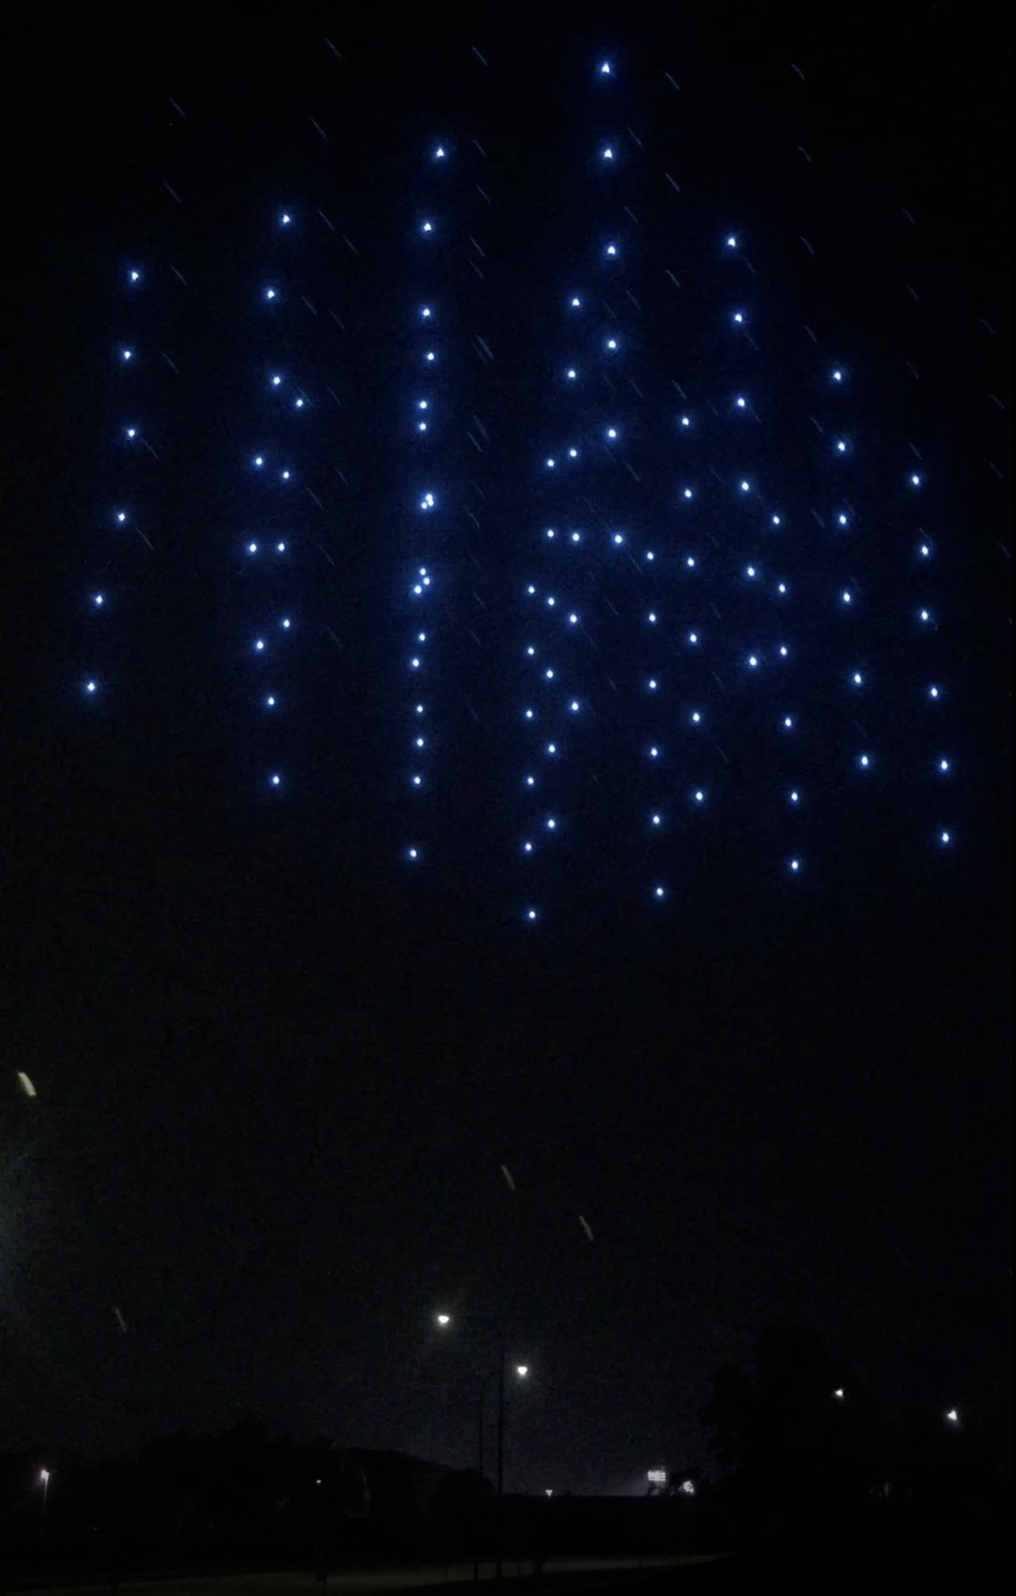
\includegraphics[width=\linewidth]{figs/firefly.png}
\end{minipage}
\begin{minipage}{0.55\columnwidth}
	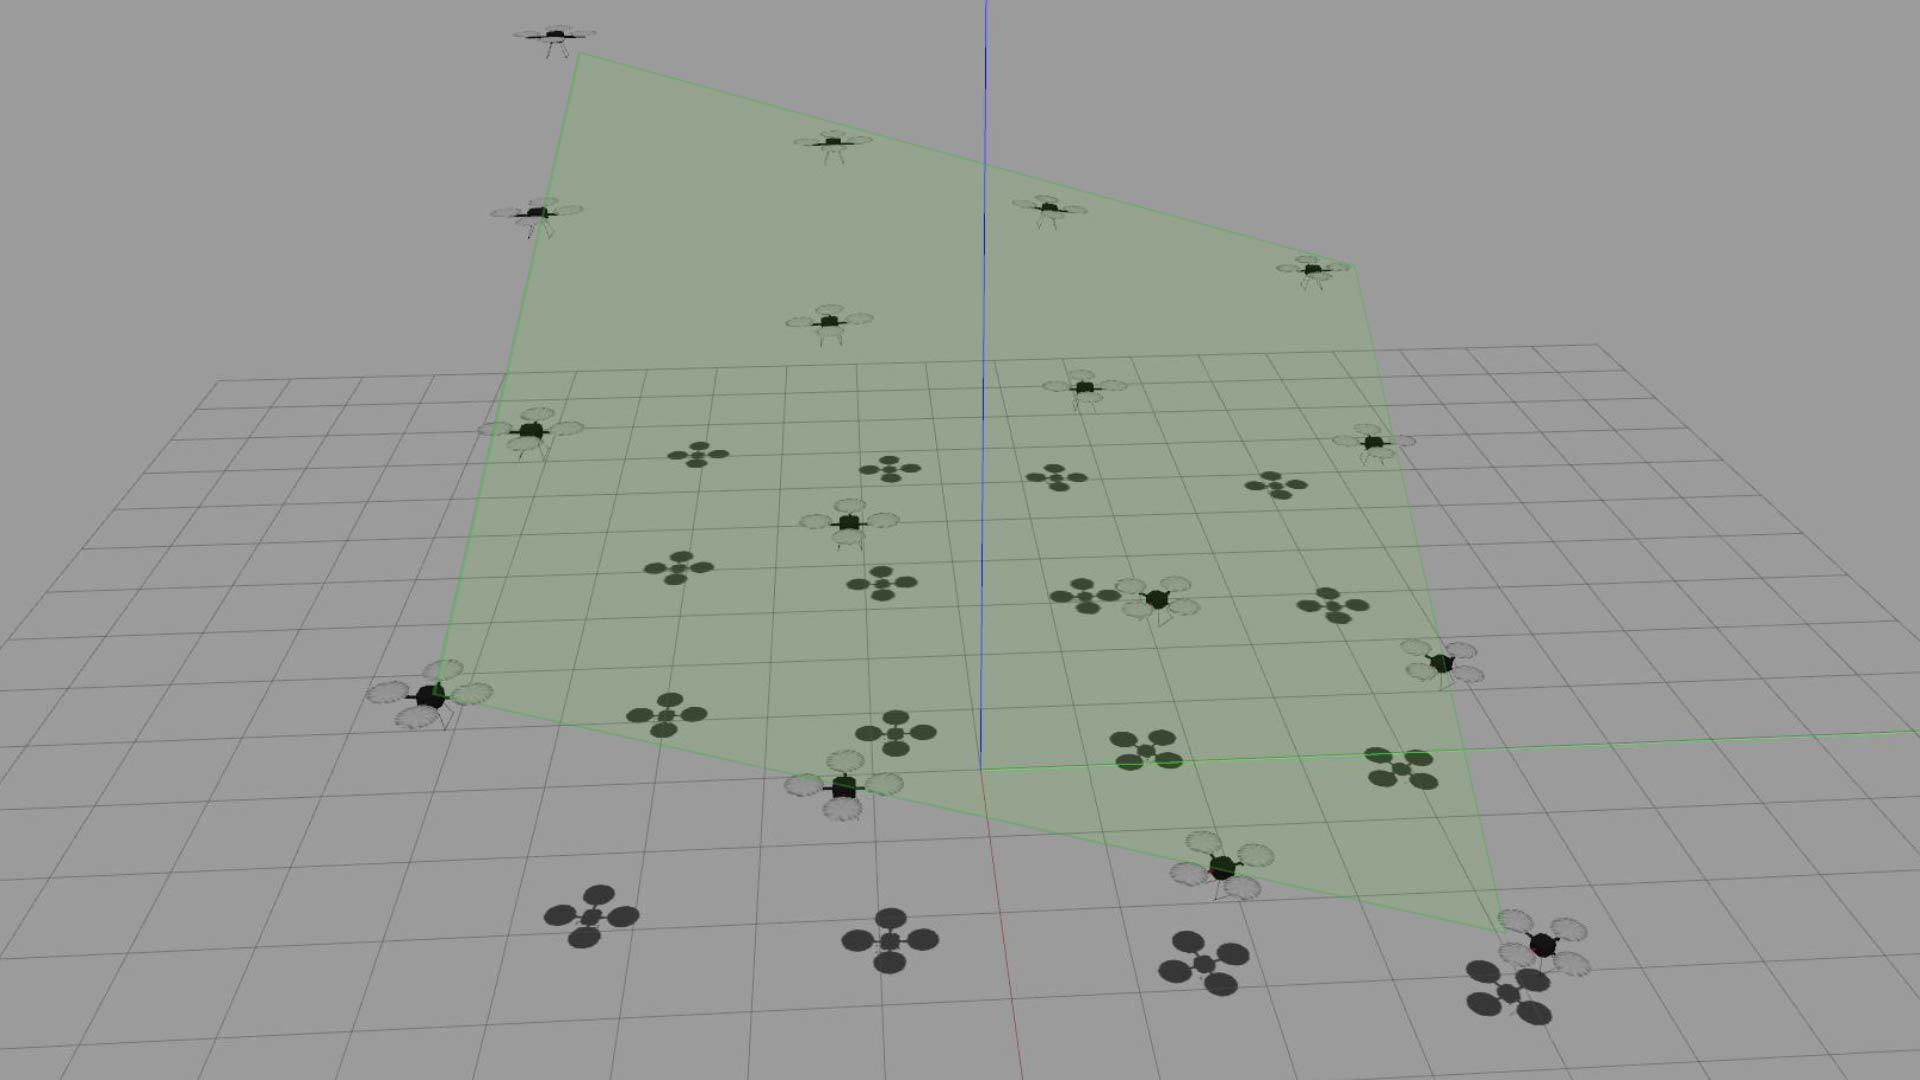
\includegraphics[width=\linewidth]{figs/shapeform_16.jpg}

	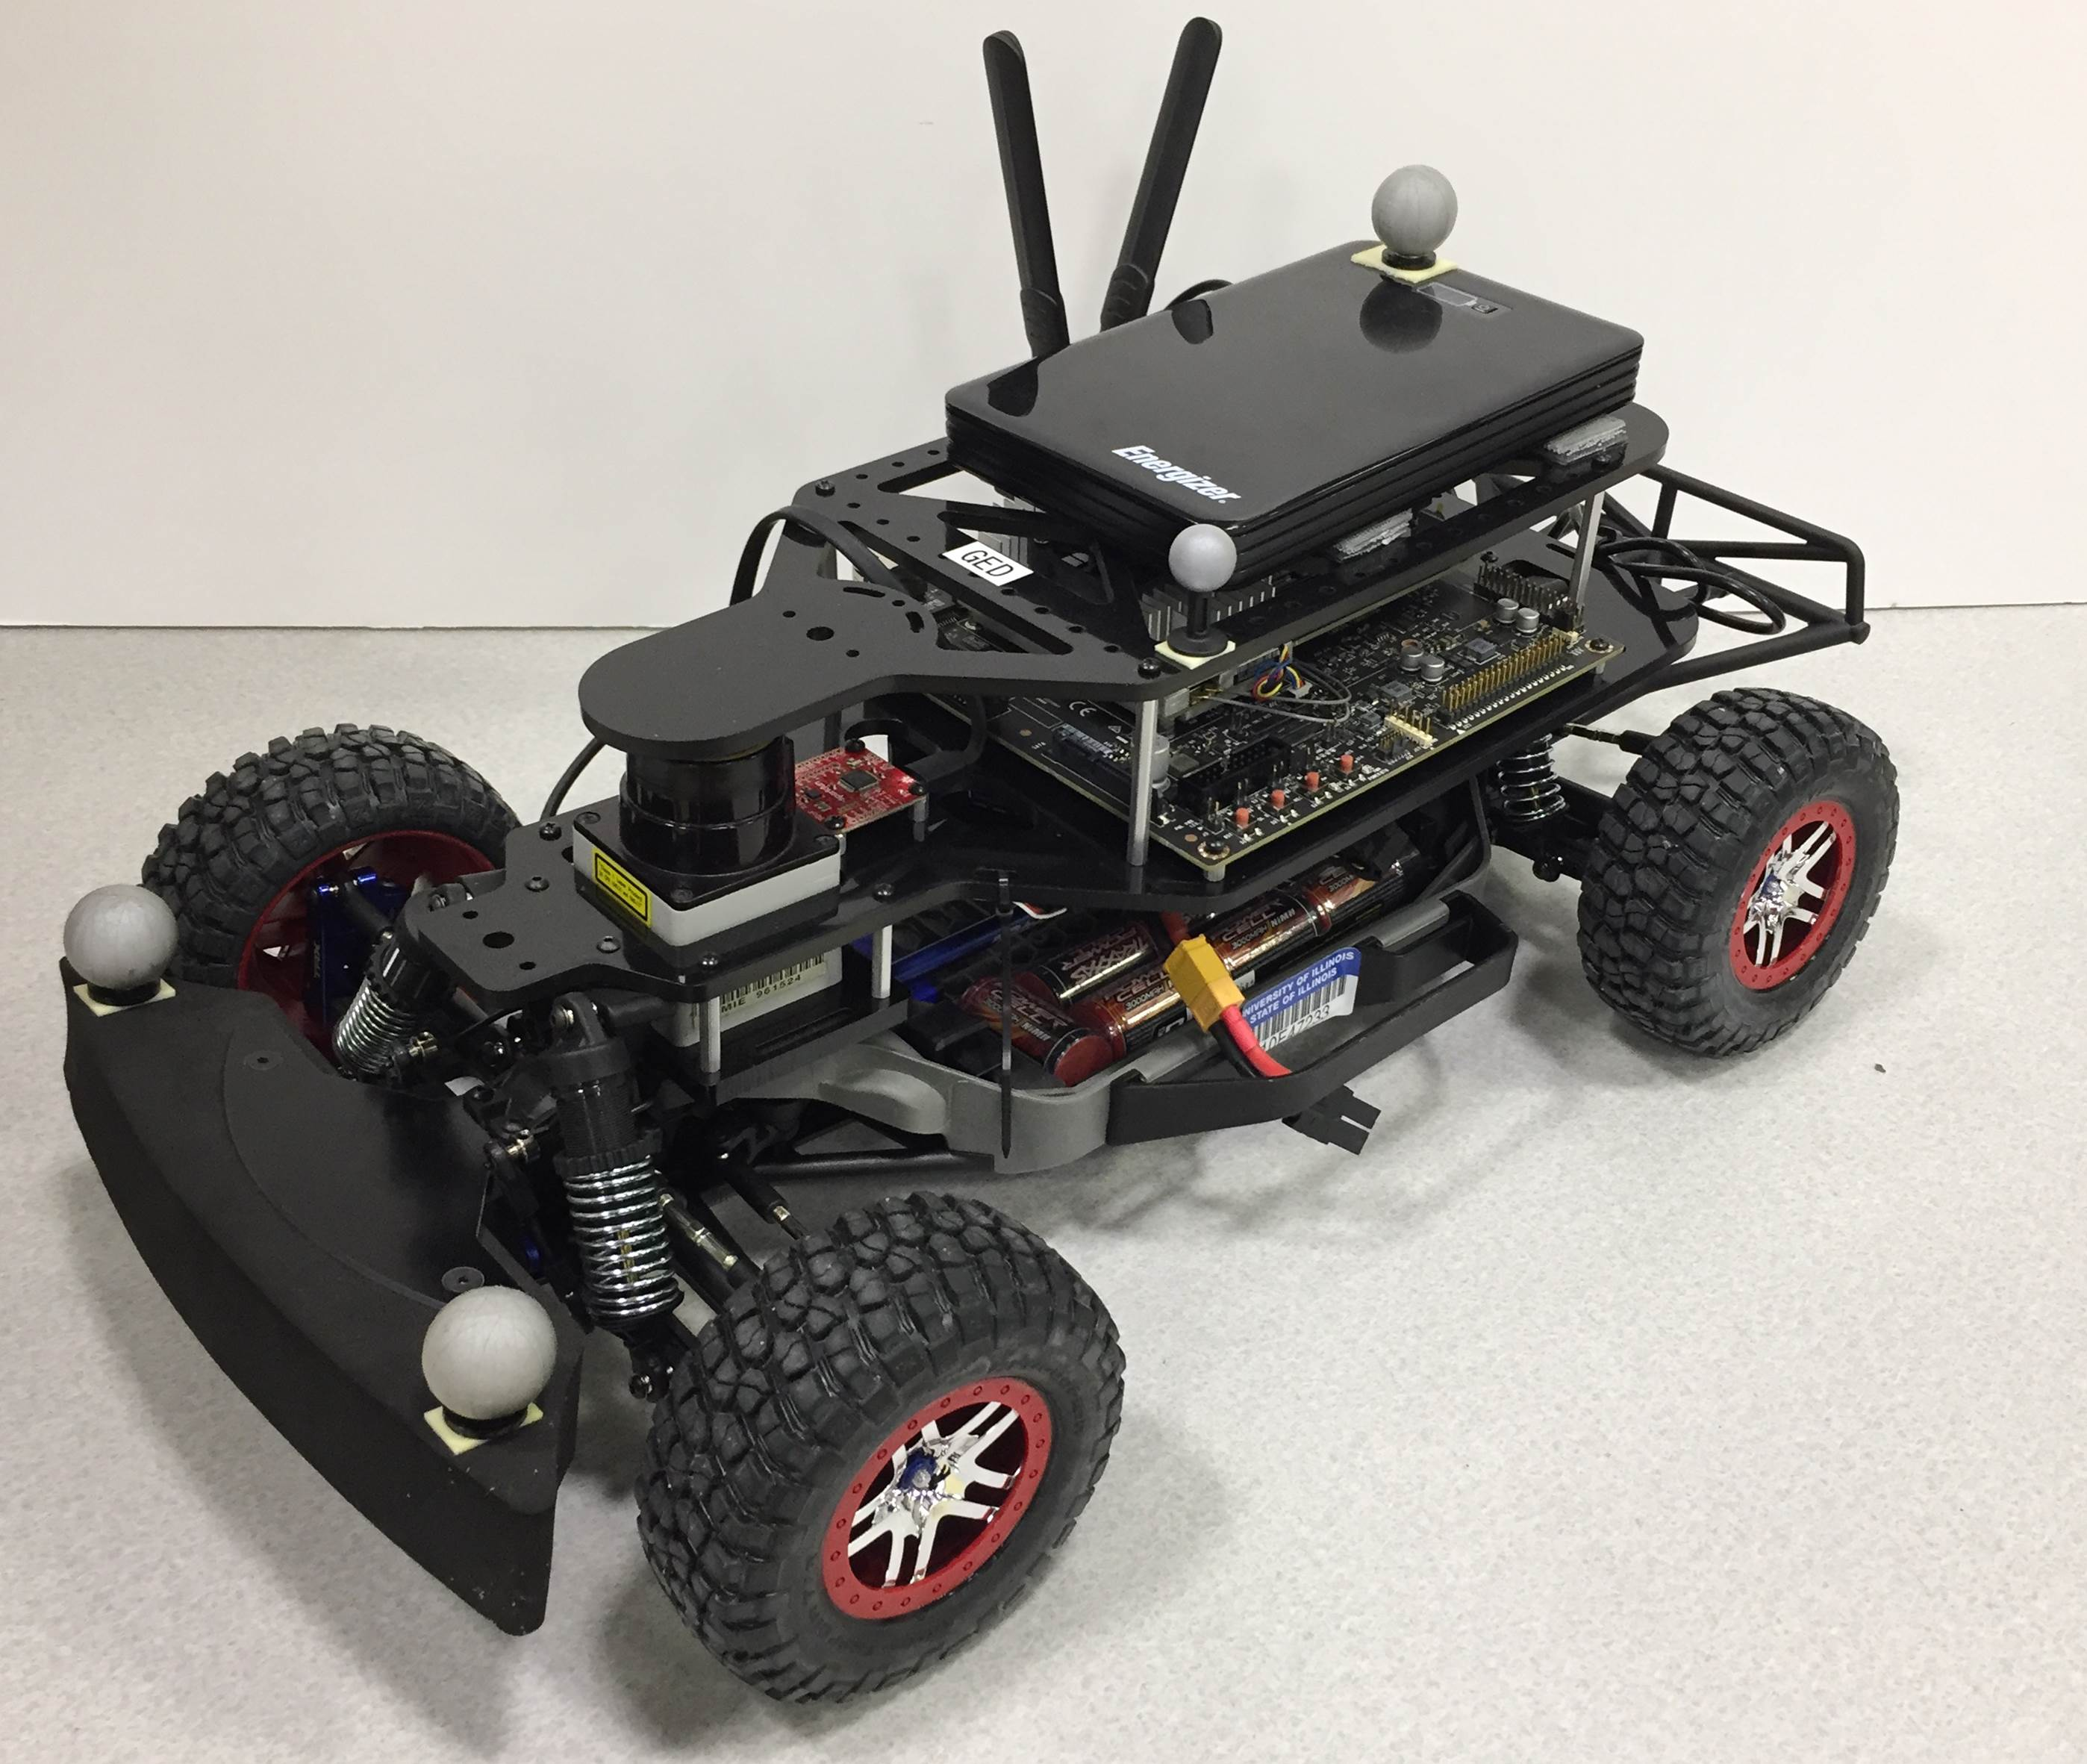
\includegraphics[width=0.4\linewidth]{figs/car.jpg}
	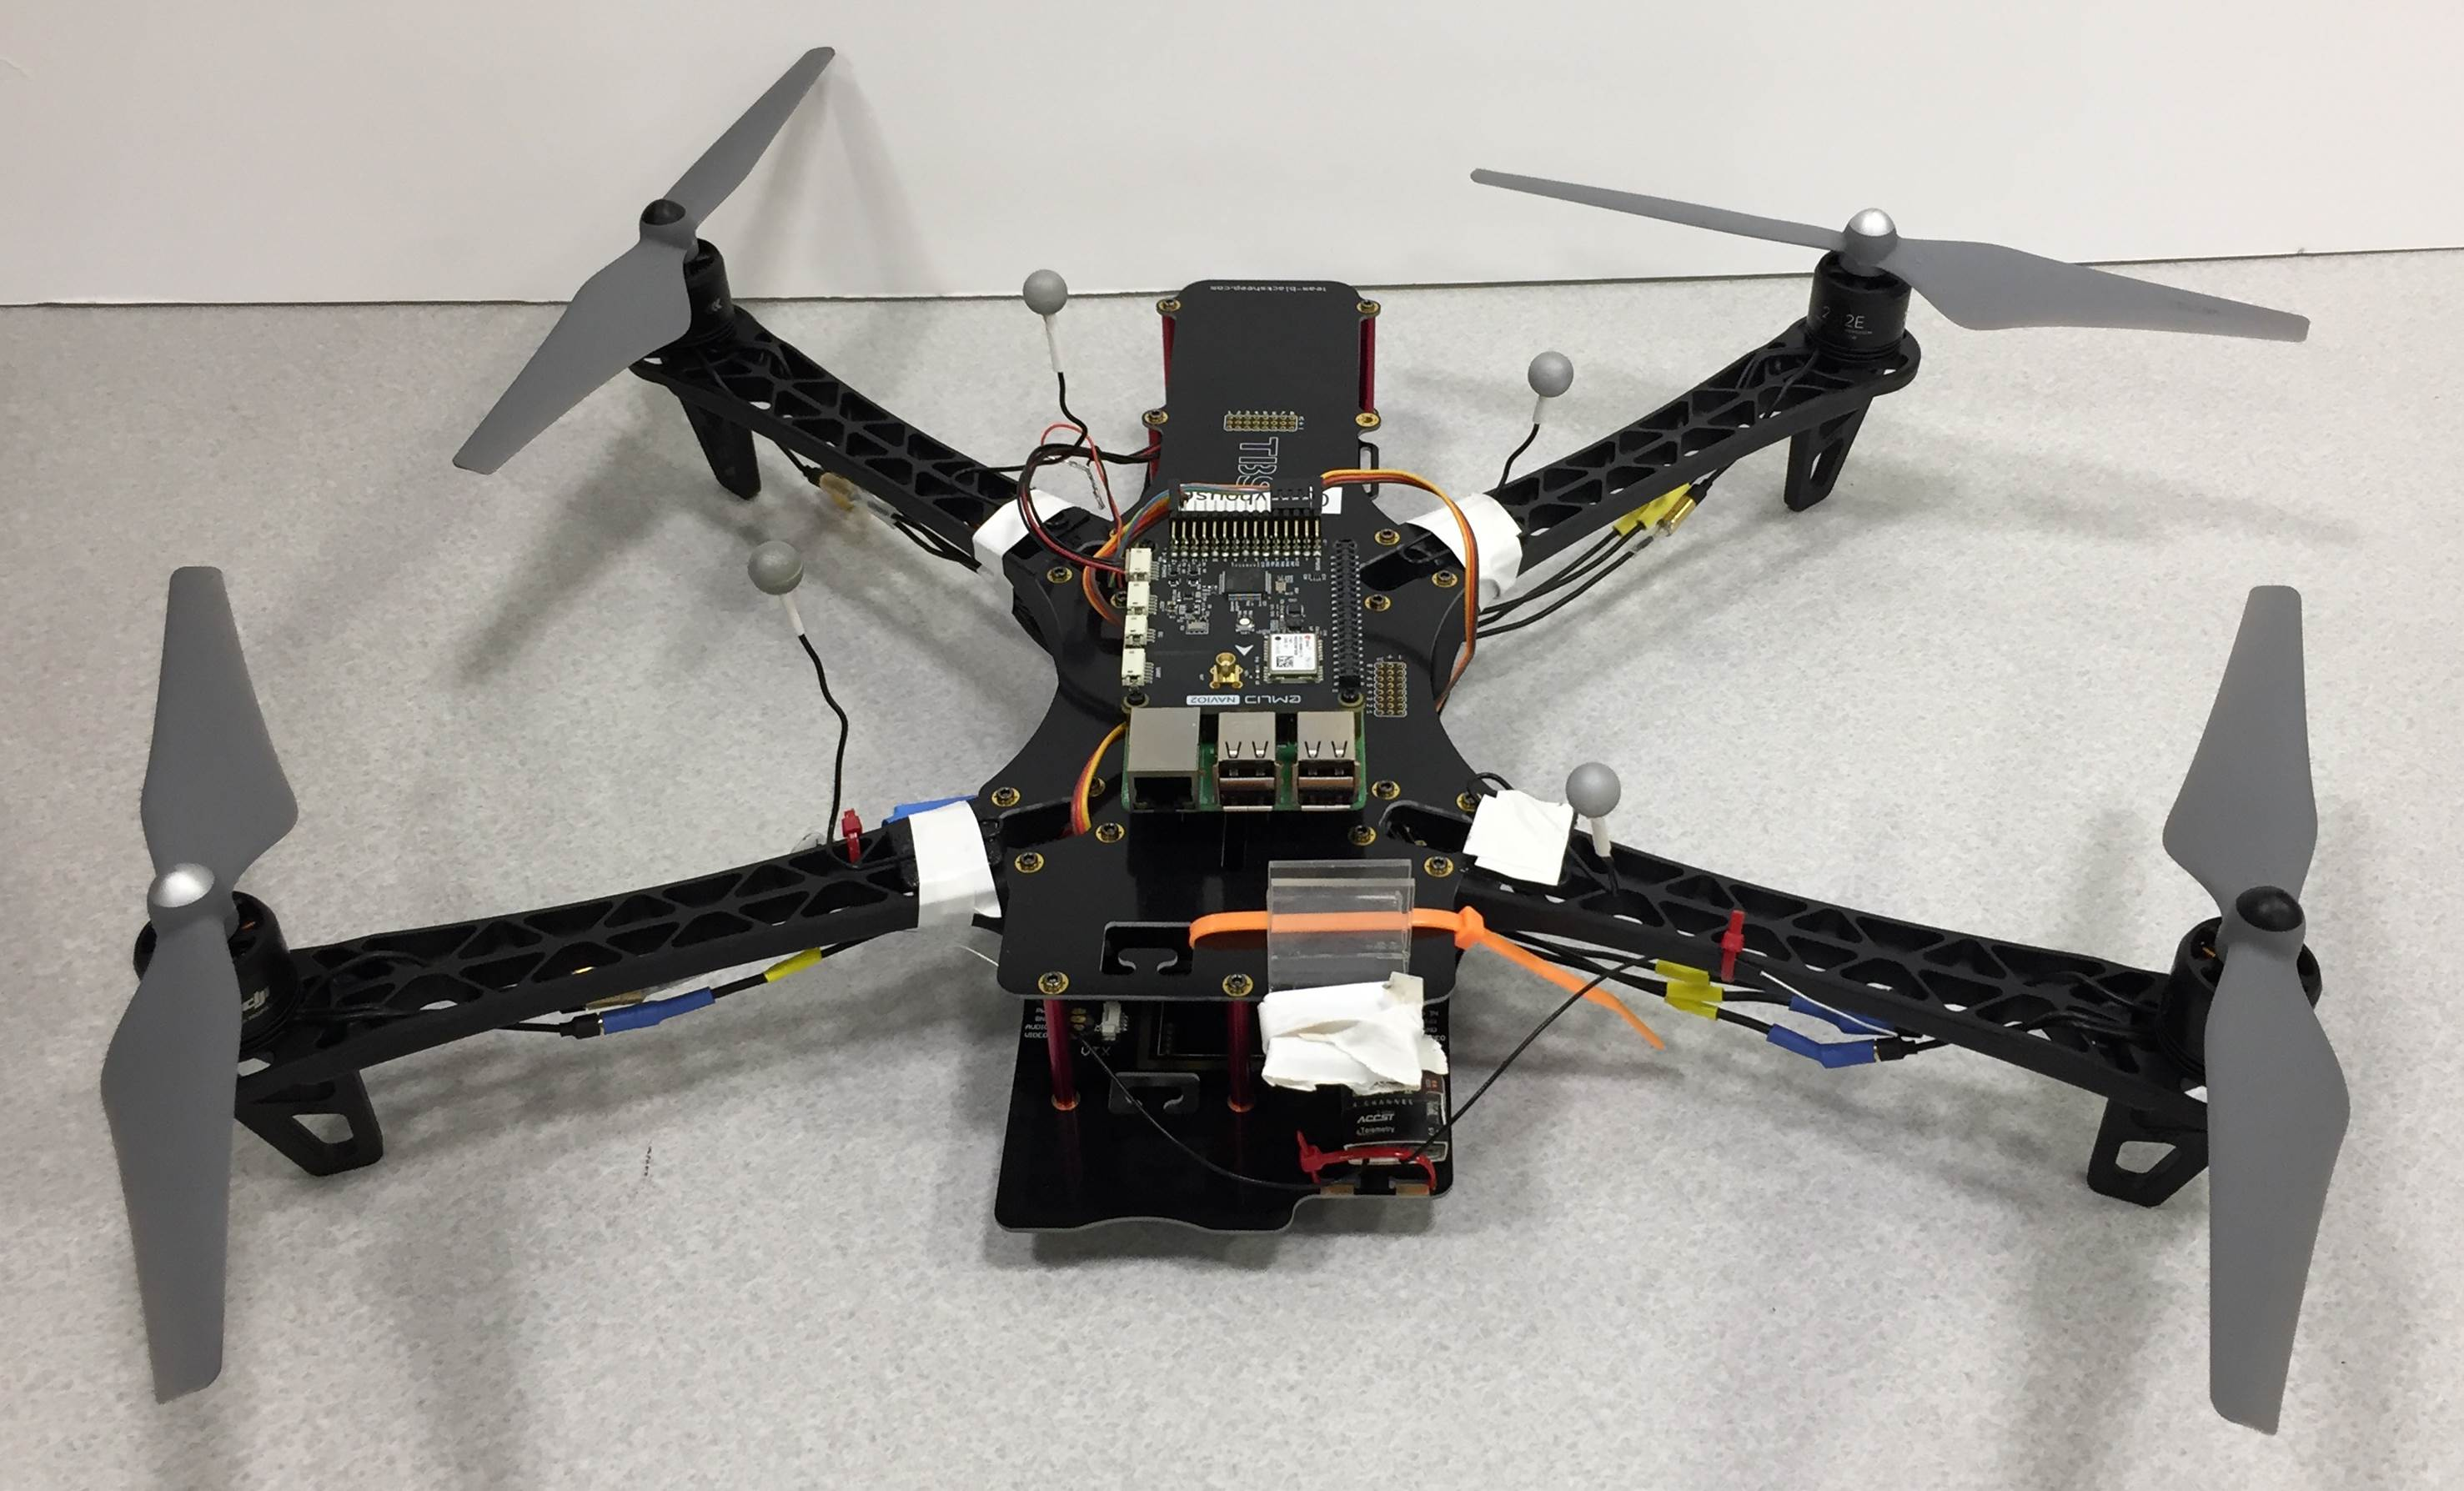
\includegraphics[width=0.55\linewidth]{figs/quad.jpg}
\end{minipage}%
	\caption{Swarm formation show by FireFly Inc. (\emph{Center}). Simulation of shape formation (\emph{Right}).}
    \label{fig:firefly}
\end{figure}

\paragraph{Implement trusted run-time environment}

\rg{Outline implementation issues }
\sayan{SM:Top of page 2/3 should have the end-to-end figure. Algorithm-code-simulator-deployment.}

[EuroSys'17] An Empirical Study on the Correctness of Formally Verified Distributed Systems.
One root cause for the bugs is because the assumptions over the underlying run-time environment. Even the systems is formally proven.

Synchronization, Timing, multi-threading, controllers, sensor fusion:
motivates nailing down exact assumptions for any sort of guarantee.

Need to validate that the abstraction over continuous time is realistic.
Why we can really use the model of zero time computation and delta time environment turn.

Need to validate the assumptions over black box parts


\begin{figure}[h!]
\centering
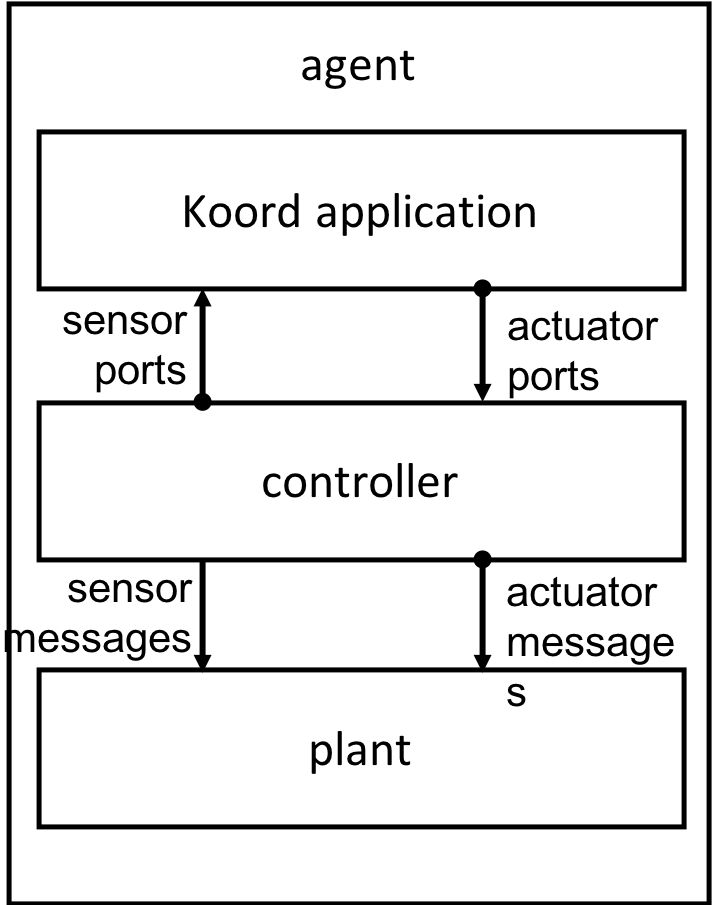
\includegraphics[height=5cm]{figs/arch.png}
\caption{\toolname framework.}
\label{fig:arch}
\end{figure}

\subsection{Contributions~\chiao{(<= 0.5 page)}}
An application deployed to heterogeneous devices and runs reliably.
This is cool and difficult to achieve without our contributions.
\begin{itemize}
\item Koord, an event-based language for modeling distributed CPS
\begin{itemize}
\item Formally specified execution semantics in K for discrete distributed part with synchronous shared memory model
\begin{itemize}
    \item Abstract away continuous time in language while provide guarantees by the carefully designed memory model
\end{itemize}
\item Simple (and formally defined?) interfaces to interact with black-box modules thru sensor/actuator variables for continuous dynamics
\begin{itemize}
\item Separate device-specific from device-independent
\item Trade-off between exposing more low level details and simplicity of the language
\end{itemize}
\item Enable (manual) formal analysis (for example, on DMap or Task)
\begin{itemize}
\item Expose assumptions over the black-box modules that need to be satisfied for proving
\end{itemize}
\item Difficulties: All of the above have to deal with time. Eg., cycle time in synchronous communication, sensor sampling frequency, synchronize data from different sensors (sensor fusion), etc.
\end{itemize}
\item  A compiler translates Koord to Python and a device-independent middle-ware implements the memory model and module interfaces
\begin{itemize}
\item Achieve distributed shared memory thru round base synchronous message passing
\item Convert pub-sub based message passing to black-box module interface
\begin{itemize}
\item Allow configurations to use different device-specific implementations
\end{itemize}
\end{itemize}
\item A Gazebo based simulation environment for testing (and data driven verification?)
\begin{itemize}
\item Wrap around black-box modules (ROS packages) to satisfy assumptions identified in formal analysis : Most technically challenging but difficult to sell
\item Visualization
\end{itemize}
\item \sayan{An intended useful outcome of this methodology  is a list of formal assumptions for the \sayan{sensors, schedulers, ...}. In the end-to-end safety assurance cases~\cite{} for complex cyber-physical systems, these assumptions  can serve as contracts for sensing devices, drivers, hardware platforms,  and operating system modules that are often outside the control of the application programmer.}
\item Finally, \sayan{experimental evaluation. What did we learn that can generalize beyond this specific application? How did we extend CyPhyHouse capabilities generally?}

\end{itemize}

%The application program \dmap is X lines of \lgname code with a \sayan{handful} external functions.
%%
%The application program, takes full advantage of the \lgname language's features shared memory semantics.
%Individual robots update their local maps using LIDAR scans, and a \sayan{single line of \lgname code} merges the local maps to update the shared global map.
%\sayan{Similar sentence about path planning and sensing.}
%
%
%Second, the modular structure and semantics of the \dmap application makes it possible to formally reason about its correctness. We illustrate this by proving key correctness and consistency properties of the application, namely that, \sayan{write informally.}
%%
%


%Define abstraction for sampled sensing. (refine this)










%The simulator enables the user to test their discrete event loop with simple motion models to test and debug the application program logic without incurring the cost of hardware deployment in case of buggy programs.
%The simulator also serves as a visualization tool as it can be used to plot the behavior of any program variables, or controller variables. For instance, we implemented a robot \emph{formation} app in $\lgname$, where several robots form a shape in which they are evenly distributed.






%\subsubsection{Other by-products}


%Design and development of the CyPhyHouse open source software system. This includes a discrete event simulator for distributed robotic systems, the application launcher, the run-time logging and monitoring system, and an integrated indoor positioning system. All of these software tools are integrated with our new robot programming language called $\lgname$ and its compiler.





%Design and development of the Koord programming language and the supporting verification tool KoordBMC~\cite{koordreport}--- significant, related but separate efforts---are not contributions of the current paper; we discuss their usage for the sake of completeness.
% completely describing the framework.
% the Demonstration of an example application development using CyPhyHouse tools and deployment on a physical system using multiple quadcopters.
%Non-contributions: Spell these out  to avoid misdirected criticisms and conflict with overlapping publications.
%\begin{itemize}
%\item Language design
%\item Verification tools.
%\item Low-level controller design for vehicles.
%\end{itemize}

%\begin{figure}[h!]
%\centering
%\includegraphics[width=0.45\textwidth]{figs/exp_traces.png}
%\caption{\small Experimental run in our testbed. The traces show the path of each robot for the last $2$ seconds. }
%\label{fig:exp_traces}
%\end{figure}


